\chapter{Application Development} \label{chap:chap5}

\section*{}

This chapter covers in detail the development phase for the application, starting with the suggestions obtained in the performed focus group to evolve the initial drafts all along to the implementation phase. In the section \ref{interfacecon}, that process will be described, concept by concept.

\section{Architecture}

\subsection{Data Model}

The data model for this application was initially the same conceived and referred in \cite{kn:Gonc12}. That said, it carries the same assumptions and limitations then assumed, such as the simplified network concept (where a network is not centred in the user, as desired for the future, but represents a single line and direction).
Therefore, checking-in in a network represents sharing information with other users in the same line or direction, where it should represent sharing information with users performing trips in a set of routes, lines or directions with relevance to the pair origin-destination where the user checked-in.

The same data model was refined in a second iteration of the project, aiming to give additional intelligence to the application, by calculating relevant routes for a given origin and destination. The relevant routes are calculated through inferring from past data from validations supplied by \emph{STCP}, and users in routes considered relevant are due to be added to the initial user temporary network (the same who provided the origin and destination used to perform that calculation) \cite{kn:Dia13}.

The refined data model introduced another change: the usage of transport public data from the city of Porto, while the older one used data from \emph{Transports from London}(TFL), which were used in the tests performed in the field among users. 

In this work, some adaptations to this recent version of the data model were made, in order to allow some concept modifications. Those adaptations will be mentioned and explained in the following sections, along with the reasons that lead to them.

\subsection{Android Application}

As said before, the technology chosen for the functional prototype of the application is \emph{Android}. This choice was made due to several reasons. 

The first reason is portability. \emph{Android} applications are developed in \emph{Java} (although, a modified version of \emph{Java}, along with \emph{XML}). \emph{Java} code is compiled to run in any Java virtual machine, making it possible to develop applications in any environment, either it is \emph{Windows}, \emph{Linux} or \emph{Mac OS}.

The choice about target version has fallen on the \emph{Ice Cream Sandwich} API, which, as mentioned in section \ref{technology}, has several advantages regarding UI design and implementation and interaction patterns. 

This choice was reinforced by an additional point: Android Cloud to Device Messaging Framework, that allowed push notifications to be sent to the application. Those notifications would allow the rating feature as it was conceived previously, prompting 2 random users from a network to rate a submitted comment from that network. However, Cloud to Device Messaging Framework (C2DM) has been deprecated in July 2012, being replaced by a new service, Google Cloud Messaging (GCM).

If the maintenance and refactoring of the code that made that rating feature work in the previous application (and webservice) was a point in favour of adopting \emph{Android} 2.2 for the implementation of the application, that change (allied to the already pointed limitations of the existing rating system), were strong points against it.

\subsection{Webservice}

The webservice connecting the existing database (as well as other data concerning the route relevance calculation) and the mobile application was also the same developed in \cite{kn:Gon12}.

Similar to what was said about the data model, it was made an effort to integrate, when possible, the existing webservice with the new application prototype. However, some concept and feature changes required changes to the webservice as well. Those changes will also be mentioned in the following sections, when explaining what lead to them.

\clearpage

\section{Interface Elements and Concepts}\label{interfacecon}

This section will cover the evolution of the interface and interaction of the application during the design phase, as well as a detailed explanation about how the implementation of the designed interface was made.
All the design guidelines and examples that were in the origin of design choices are also explained. However, it must be said that usability guidelines rarely consist in hard and fast rules, and usability questions frequently don't have just a single answer. In most cases, there are design trade-offs that must be considered \cite{kn:MobileUsab}.

\subsection{Branding}

Despite being an application directed to the public, or intended to be in a near future, the attribution of a name or image associated to it was missing or yet to be discussed.


In a discussion with Eng. António Nunes, the creator of the idea behind the project, some thoughts and suggestions about a possible name for the application came up. For this iteration of the project, one of them (proposed by him) was selected - Journata.

This name was selected because in the opinion of the people involved in the project, it could give the user an initial perception about some of the application features - it can be considered a travel journal in some way - while performing a word play with the words "journey", "journal" and "data". Even the name itself, Journata, resembles the Italian and Portuguese words for "journey" - \emph{giornata} and \emph{jornada}, respectively.

Some thought was also put in creating a logo for the application. The main idea was to resemble a public transport vehicle (bus or subway), while giving a modern look to the referred vehicle and to the logo itself. In the following figure, it is possible to find the designed alternatives for a first logo of the application. 

\begin{figure}[htb]
  \begin{center}
    \leavevmode
    
\includegraphics[scale=0.2]{logo_versions.png}
    \caption{Application first logo alternative designs.}
    \label{fig:logo}
  \end{center}
\end{figure}

The middle option was then selected to be part of the prototype.


\subsection{Main Navigation}

After the realization of a focus group session (see section \ref{focusgroup}), the design choice had fallen over a tab navigation, consisting in four tabs, always visible.

Those tabs were meant to represent:

\begin{itemize}
\item News Feed
\item Comment Submission
\item User Profile
\item Journey Planner
\end{itemize}

The design decision about the existence of text labels as an additional information (along with suggestive icons) was made in order to make the learnability of the interface easier. There are several well-known mobile applications who use tabs as their main navigation component, and social networks are no exception. In the following figure, it is possible to see a screenshot of the \emph{Facebook} application for \emph{Android}. 

\begin{figure}[htb]
  \begin{center}
    \leavevmode
    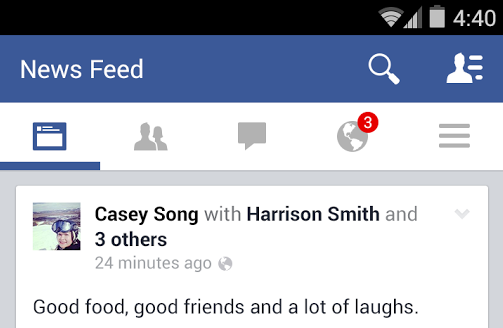
\includegraphics[scale=0.6]{facebook1.png}
    \caption{Screenshot of \emph{Facebook} application navigation component for \emph{Android}.}
    \label{fig:facebook1}
  \end{center}
\end{figure}

Here, it is possible to see that the chosen navigation does not have text labels with additional information about the features they refer (in some cases, textual information about the feature can be seen in the Action Bar, though). However, in this case it is considered acceptable, since \emph{Facebook} users know the displayed icons very well and associate actions and meaning to them, since the same icons are displayed in the \emph{Facebook} website for years and users know pretty well what the actions associated to them (preserved in the mobile application).


A distinct example can be \emph{Swarm}. This recent application, from the creators of \emph{Foursquare}, has a tab-based navigation as well, but because users are not yet familiar with the features associated to those icons, there is an initial difficulty in the application learning process.

\clearpage

\begin{figure}[htb]
  \begin{center}
    \leavevmode
    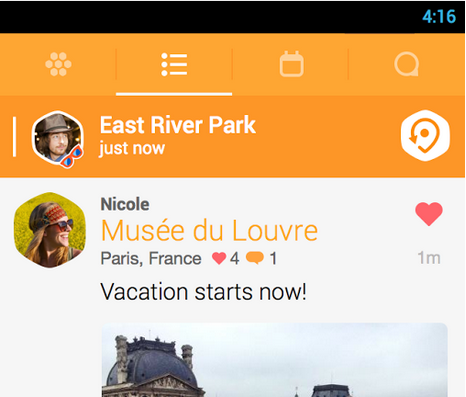
\includegraphics[scale=0.6]{swarm1.png}
    \caption{Screenshot of \emph{Swarm} application navigation component for \emph{Android}.}
    \label{fig:swarm1}
  \end{center}
\end{figure}



Other reason to provide textual information labels along the icons is the widespread usage of those labels in \emph{iOS} applications, where tab navigation is fairly common, despite being in the bottom of the screen.

\begin{figure}[h!]
  \begin{center}
    \leavevmode
    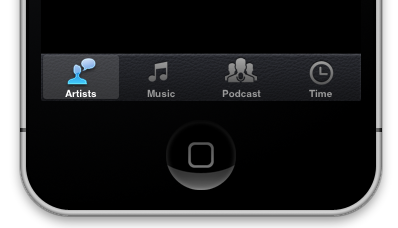
\includegraphics[scale=0.6]{ios_tabs.png}
    \caption{Example of a tab navigation in an \emph{iOS} mobile application.}
    \label{fig:ios-tabs}
  \end{center}
\end{figure}


\subsubsection{Iterations}

One of the first decisions after the focus group was to re-order those tabs by perceived importance. The information in user profile was perceived as less important than the journey planner features (or at least it is intended that the journey planner features have more visibility). To accomplish that, the journey planner tab was then moved to third place (from left to right), switching its place with the user profile tab.

The label associated to the journey planner tab was also changed in order to inform the user that that tab included some more features but not just the planner, such as a list of favourite and scheduled trips.
It is possible to see the result of that decision in figure \ref{fig:mainnav3}.


\begin{figure}[h!]
  \begin{center}
    \leavevmode
    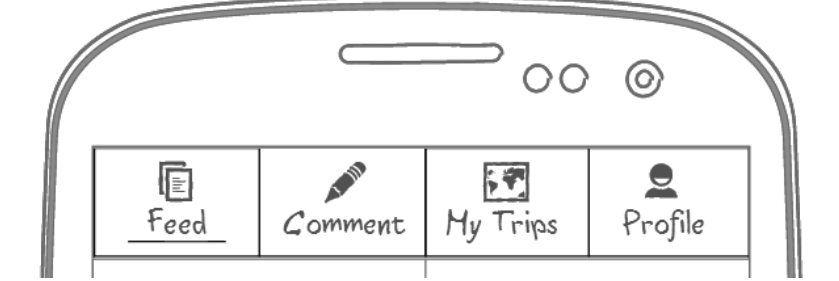
\includegraphics[scale=0.6]{mainnav3.png}
    \caption{Second iteration of the tab navigation interface.}
    \label{fig:mainnav3}
  \end{center}
\end{figure}

This new version of the interface was not changed until the end of the design phase, when it was the subject of an usability test along with the remaining components of the interface(see Appendix \ref{ap2:usabtest}) and consequently validated.

\subsubsection{Implementation}

In the implementation of this component, an external library (ViewPagerIndicator \footnote{\url{http://viewpagerindicator.com/}}) was used and customized in order to facilitate the integration of swipe gestures to alternate between tabs. This way, a more fluid interaction was made available to the user.

The \emph{Android} Action Bar was also used, despite not being part of any of the interface design, to include elements such as the application name, logo and an option menu with features missing in the design iterations.

\begin{figure}[h!]
  \begin{center}
    \leavevmode
    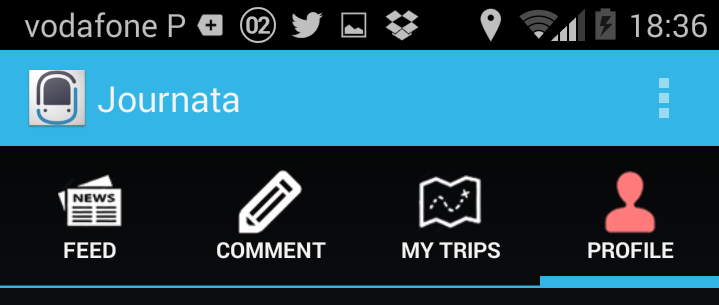
\includegraphics[scale=0.8]{mainnav4.png}
    \caption{Screenshot of the implemented application's main navigation.}
    \label{fig:mainnav4}
  \end{center}
\end{figure}

\subsection{News Feed}\label{newsfeed}

After the performed focus group, one of the suggestions consisted in the introduction of feed subscriptions. The user could receive information from several networks (instead of just one, as previously established), subscribing an information feed of each network for that matter. 

\subsubsection{First Iteration}

An initial thought on that suggestion resulted in considering the possibility of having several check-ins at the same time. The first design iteration after the realization of the focus group was aligned with this idea. Subscribing a network feed (the act of adding the subscription) therefore implied the check-in of the user in the same network. 

Four new features were then considered: 

\begin{itemize}
\item Add a new feed subscription (previously there was no need to add, since the network were the user was checked-in was the one whose information was displayed);
\item Listing the current feed subscriptions;
\item Removing a feed subscription;
\item Filter visible feed subscriptions (the 'view feed' feature would display a 'global feed', with all the feeds subscribed. With this filtering, the user could mark one or more feeds to be invisible in the 'global feed').
\end{itemize}

The need for the existence of a secondary navigation (similar to what was discussed for journey planner features in section \ref{jourplaninit}) presented itself in this component as well. For better coherence between secondary navigations in other tabs and for improved visibility of all the available options to the user, a secondary set of tabs was chosen.

To subscribe a new feed, the user would indicate the origin and the destination of the network from which he desired to retrieve information (the origin or destination could be based on the user's GPS location, searching the nearest stops), as well as the date and hour for the information. 
Then, the user would retrieve a list with several options, listing all the vehicles and methods of transportation available at the supplied date and hour. To make the list item selection easier, a button to select/deselect all the options would be available as well.

That way, if an user wanted to retrieve information between A and B, and three possible transportation methods/vehicles are available, the user would need to select all the three of them in order to get information from all those lines and perform an informed decision (see figure \ref{fig:feed_iter1_add}).

\begin{figure}[htb]
  \begin{center}
    \leavevmode
    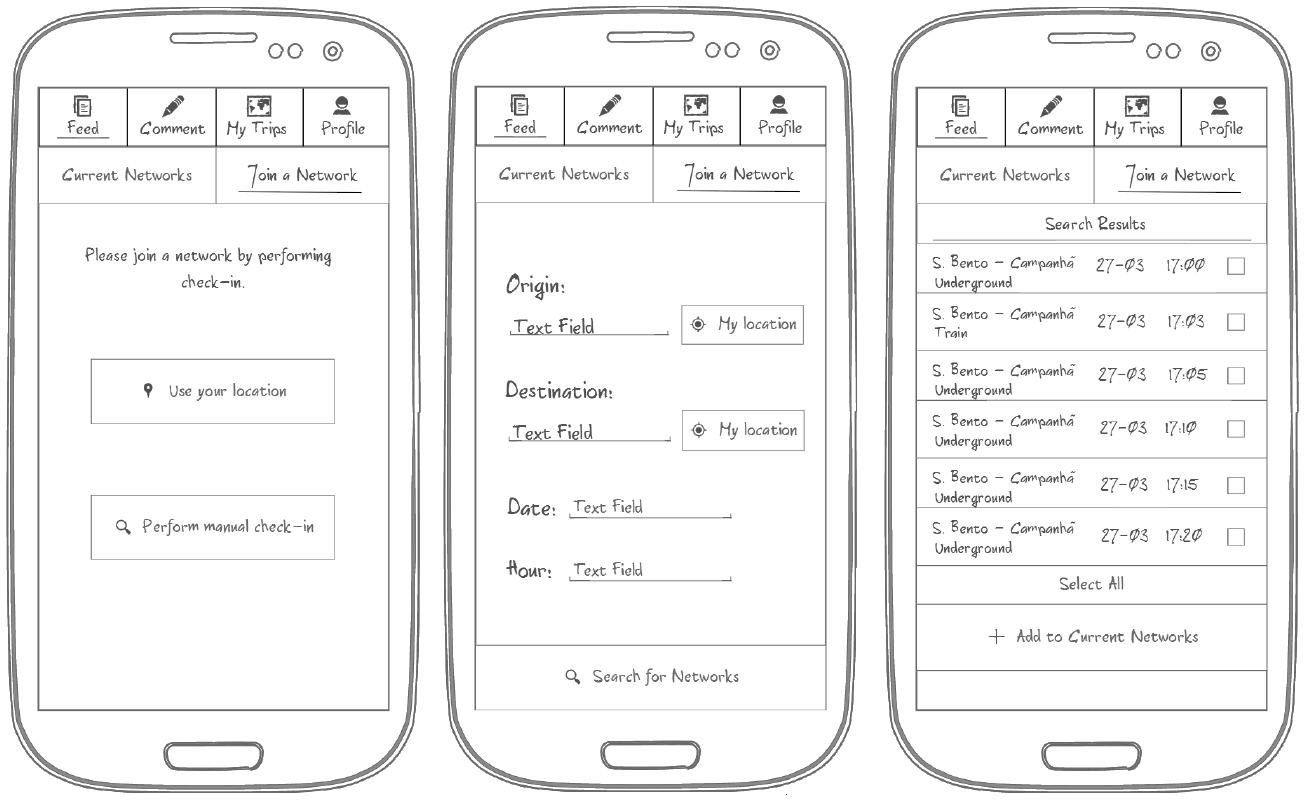
\includegraphics[scale=0.4]{feed_iter1_add.png}
    \caption{News Feed features and screens - Add Feed, First Iteration.}
    \label{fig:feed_iter1_add}
  \end{center}
\end{figure}




However, this design had several limitations. For example, the user usually has a hard time identifying the exact vehicle he's in (despite the fact that an hour on the schedule can be used to identify the vehicle, that vehicle can be running late, for instance. In case of transportation methods that have high frequency, such as subway, the difficulty of such a task is even higher).


This would also bring an additional problem - along with adding a feed subscription for every transportation method for the chosen course, the same was required for removing those feeds.
By clicking on an item of the list, representing a feed, a menu would also be available to the user, allowing him to remove a feed. When an item was selected to removal, a confirm dialog would be presented to the user. However, this is considered as something to avoid when designing mobile applications because of the additional effort presented to the user (additional interaction).

The 'filter visible feeds' feature was designed as a list where the users could mark each one of the current subscribed feeds as visible or invisible, through a check-box. However, it was considered that the use of a check-box to perform this selection was not efficient, because it was not clear enough to the user what were the practical effects of that selection and the actions triggered by it (figure \ref{fig:feed_iter1_filter}).

\begin{figure}[htb]
  \begin{center}
    \leavevmode
    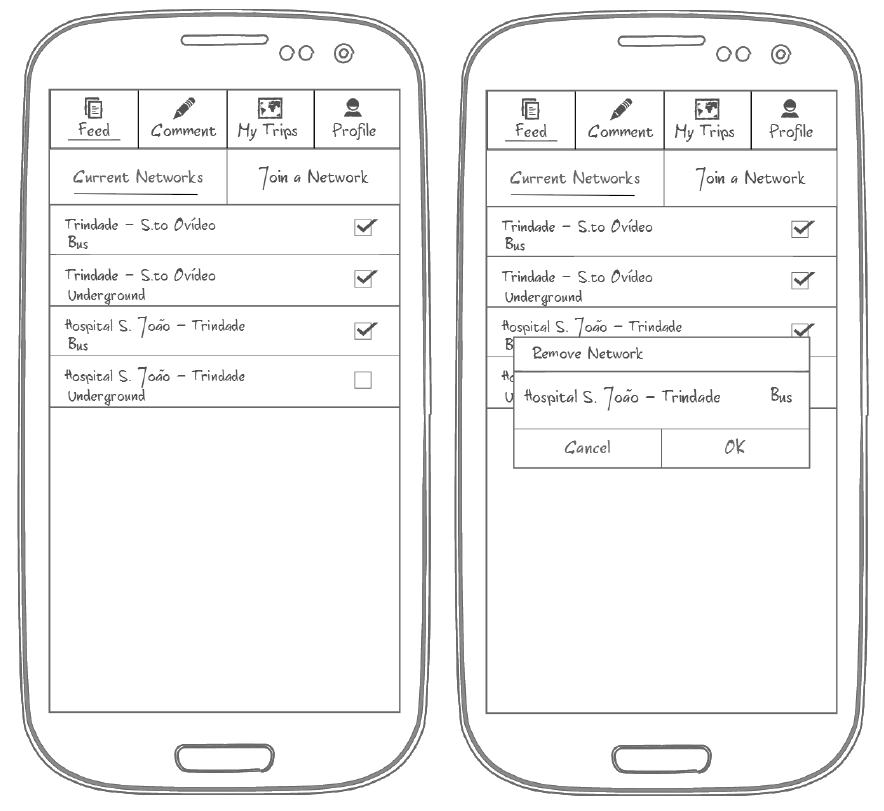
\includegraphics[scale=0.5]{feed_iter1_filter.png}
    \caption{News Feed features and screens - Filter and Remove Feeds, First Iteration.}
    \label{fig:feed_iter1_filter}
  \end{center}
\end{figure}


Viewing the news feed was considered the main and most critical feature of the application. Therefore, the need for a major redesign of this feature was recognized, because in the previous developed prototype, this feature, despite providing the functionality to the user, was not sufficiently attractive or displayed enough information to the user.

The first thoughts about this feature included what should be the information displayed to the user in each comment from a feed.
Since this was no longer a feature associated to a single route or network, every item should have the indication of the network it refers to, consisting in origin, destination, transportation method and route number (this one is only valid if it refers to a bus route).

In order to make this feature more attractive, and since between the fields available in a user profile, a photo was also considered in the initial work \cite{kn:Gon12}, an interface similar to the message display we encounter in several instant messaging or SMS sending applications for mobile devices (such as \emph{Google Hangouts}, \emph{Android} SMS application), where the user or contact photo is displayed near the content of his message.

In this case, and opposed to what was previously done, the appearance of the user's own messages along with messages from other users was conceived, in order to create that effect and to give the user a sense of contribution to the community of the users of the application, trying to improve their levels of engagement.

A different highlight color for the user's own comments was also selected, in order to differentiate them from other users' comments, and it was also conceived that those two types of comments should be aligned each one to a different side of the screen.

Each item would also have the option to give a star to the comment author, if the comment in question was considered particularly helpful. 


As said before, it was decided to aggregate the comment rating feature in the view feed screen, and the initial thought in how to do that was to highlight the items with pending user review in the top on the feed, despite possibly being older than some of the already approved comments. Those comments would also have a button that, when triggered, would prompt a dialog to the user making it possible to define and submit the rating about the referred comment (figure \ref{fig:feed_iter1_view}).

\begin{figure}[htb]
  \begin{center}
    \leavevmode
    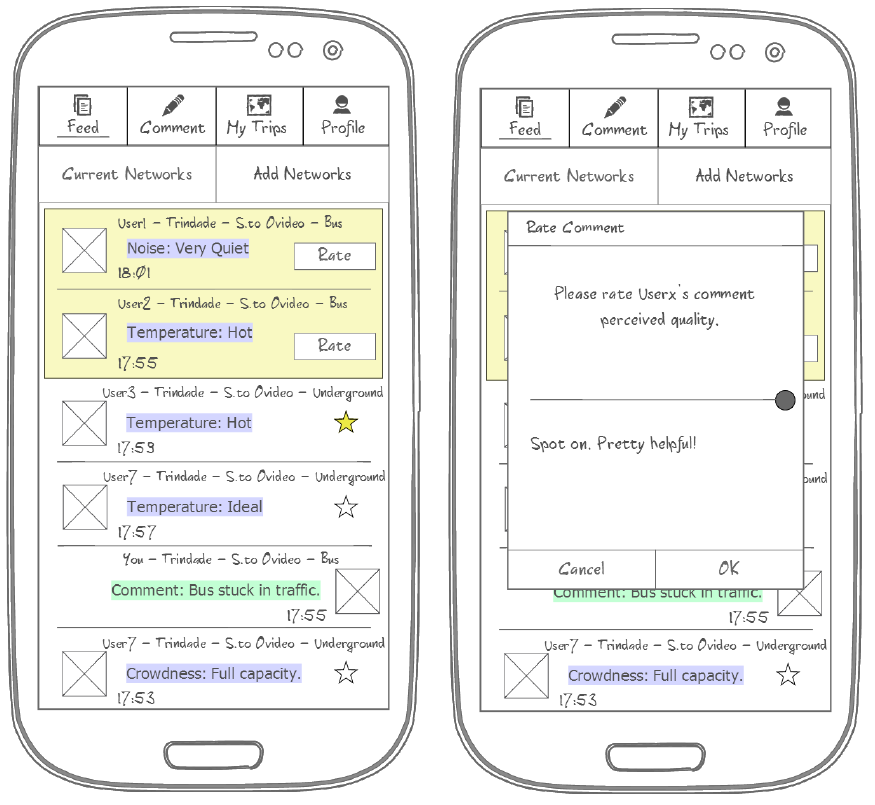
\includegraphics[scale=0.5]{feed_iter1_view.png}
    \caption{News Feed features and screens - View Feed, First Iteration.}
    \label{fig:feed_iter1_view}
  \end{center}
\end{figure}




\subsubsection{Second Iteration}

Recognising the existing limitations in the first design iteration,  a second iteration was made, based in the assumption that subscribing a network feed would be independent from check-in. This way, the existence of a check-in was not required to receive information. The need for defining date and hour when adding a new feed subscription was also eliminated.

However, the most relevant change for this new iteration was the aggregation of the feeds for several transportation methods in just one. According to this new paradigm, if the user wants to receive information between a given point A and another given point B, he would only need to subscribe one feed, defining the origin as A and the destination as B. The subscribed feed would then include all the information of all the possible routes to go from A to B, as well as other relevant routes (integrating this concept with the work developed in \cite{kn:Dia13}), independently from the transportation method. 

This way, for the previously given example, where the user has three distinct routes or options to go from A to B, the same user would subscribe an unique feed that would allow him to retrieve information from all of the three options.

The screen for adding a new feed subscription was also redesigned, having now an additional button allowing to switch the content of the text fields of origin and destination (an interaction pattern encountered on other mobile applications that present the input of similar data to the user, such as \emph{Google Maps} or \emph{Moovit}).
Several alternatives for that screen, intended to highlight and at the same time facilitate the option for choosing the current location of the user as origin or destination, were also designed (figure \ref{fig:feed_iter2_add}).

\begin{figure}[!h]
  \begin{center}
    \leavevmode
    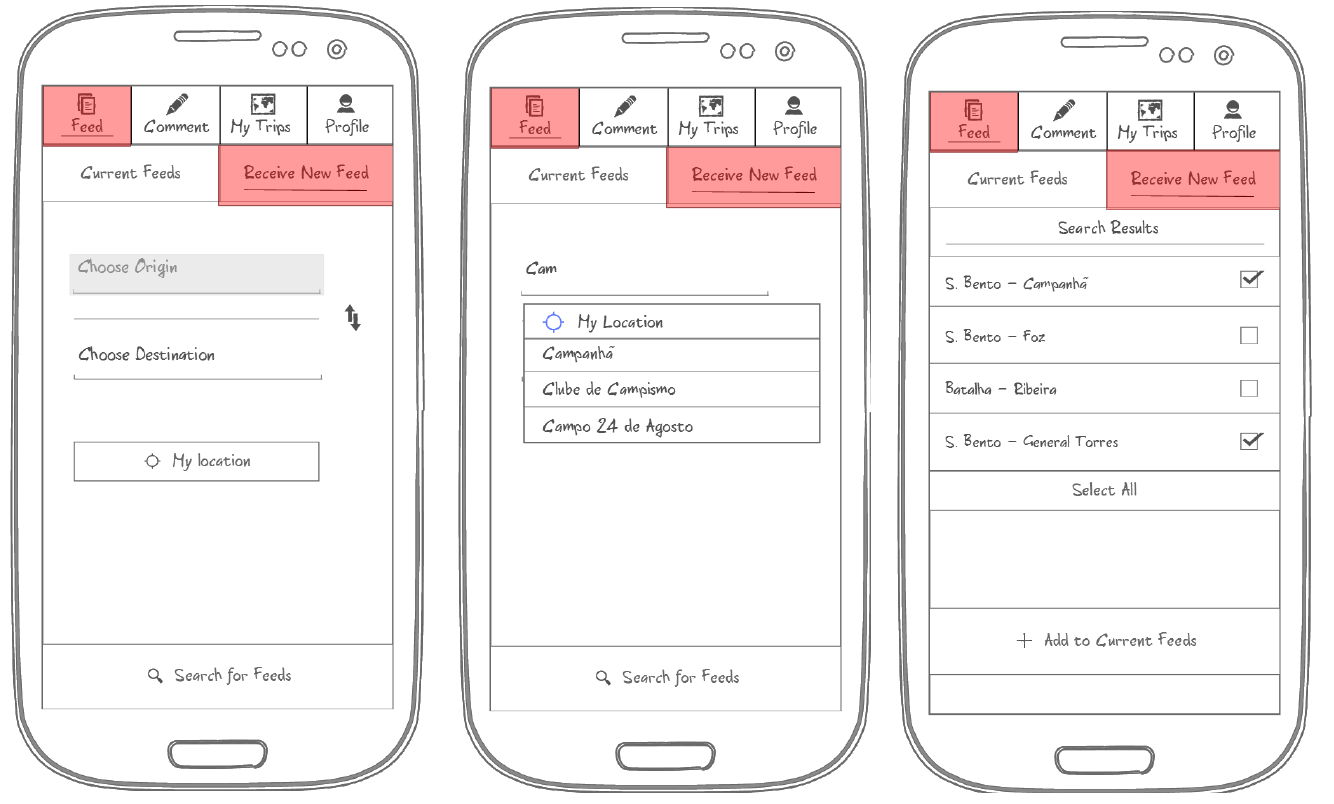
\includegraphics[scale=0.5]{feed_iter2_add.png}
    \caption{News Feed features and screens - Add Feed (alternative designs) and Search Results, Second Iteration .}
    \label{fig:feed_iter2_add}
  \end{center}
\end{figure}


Regarding the filter feeds feature, the check-box from the first iteration was replace by a switch with textual information about the feed status/action associated to it.
To the menu where it was possible to find the option to remove the feed from the list of subscribed feeds, the option to add the same feed to the list of favourites (see section \ref{journeyplanner}) was also added. 

The confirmation dialog for feed removal (or for any task at all) is considered as something to avoid when designing mobile applications. An interaction pattern that allowed to replace that sort of dialogs consists in removing the item, giving the user the option to undo the item removal for a few seconds. This pattern can be encountered in some \emph{Android} applications widely used, such as \emph{Gmail}. This interaction pattern was also considered for this feature, as it is possible to see in figure \ref{fig:feed_iter2_remove}.

\begin{figure}[htb]
  \begin{center}
    \leavevmode
    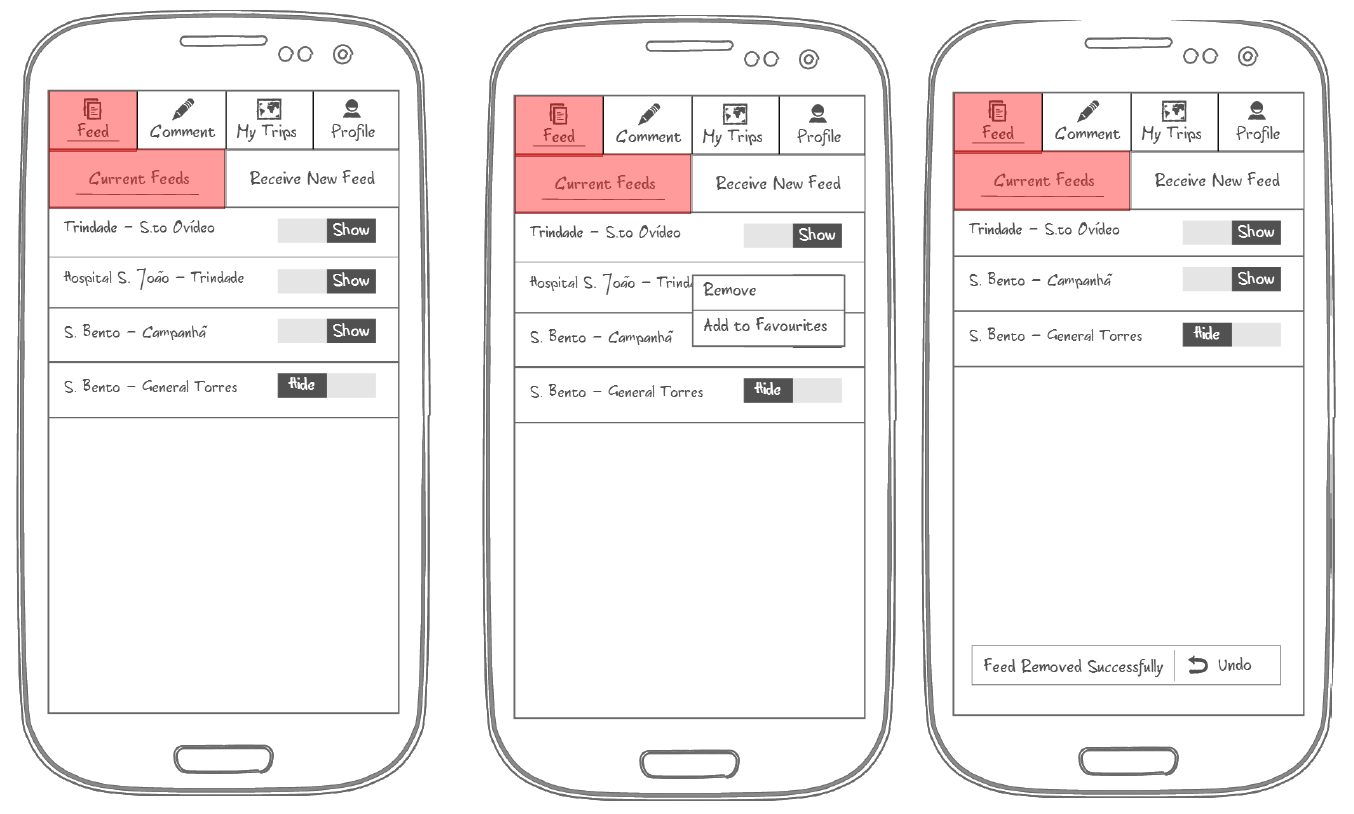
\includegraphics[scale=0.5]{feed_iter2_remove.png}
    \caption{News Feed features and screens - Filter and Remove Feed, Second Iteration.}
    \label{fig:feed_iter2_remove}
  \end{center}
\end{figure}

\subsubsection{Implementation} 

The implementation of this module of the application tried to follow as much as possible the design from the second iteration. Several screens for situations where no information was available were designed and implemented (for when the user does not have any feeds subscribed, prompting him to do so in order to benefit from the usage of the application).

One question that was not considered in the design phase was the transition between the 'View Feed' feature and the other features in this component, that had navigation between them through the utilization of a secondary navigation. For that matter, a new tab was added to that secondary navigation, in order to allow that transition and make it as easy as possible to the user (through the touch on the desired feature tab/button).

\begin{figure}[!h]
  \begin{center}
    \leavevmode
    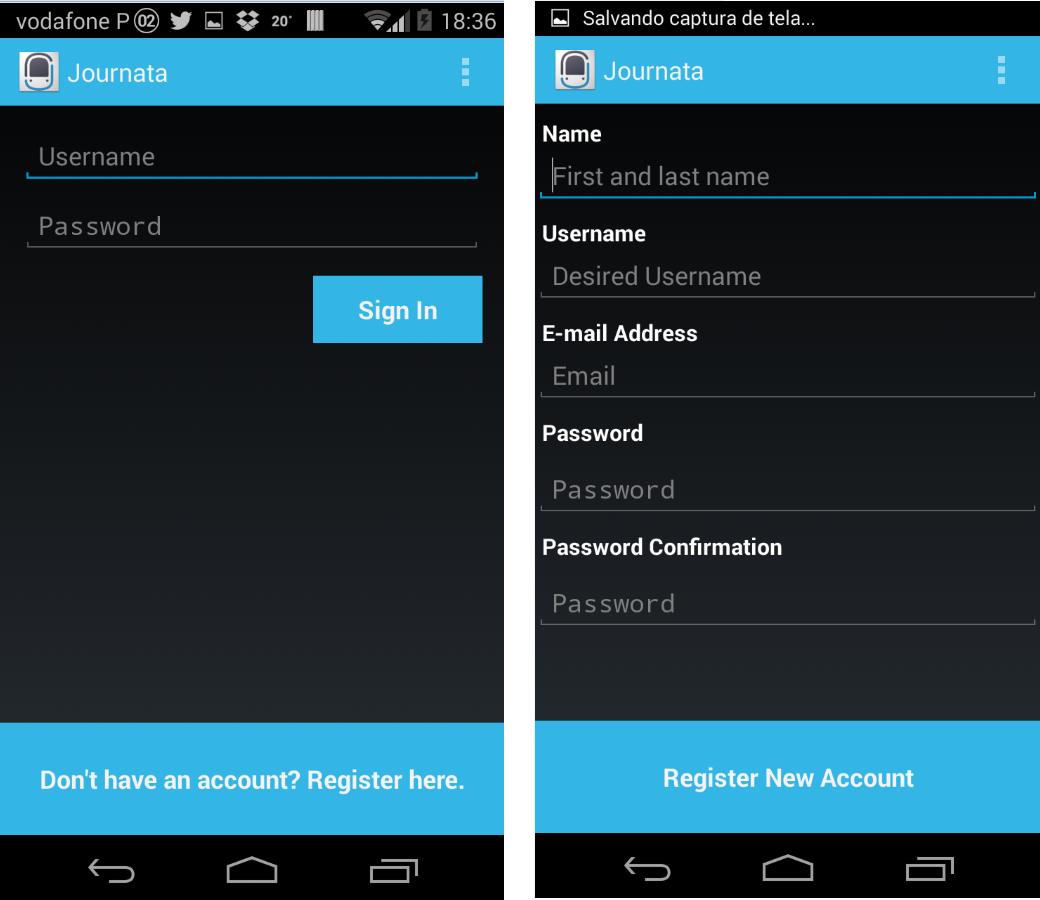
\includegraphics[scale=0.5]{login_register.png}
    \caption{Screenshots of the add and filter feed features.}
    \label{fig:feed1}
  \end{center}
\end{figure}

The form for adding a new feed used an improved version of the auto-complete used in \cite{kn:Gon12}. That was implemented in order to reduce the effort of text input from the user (it allows the user to select the desired bus stop right away). This form also allows the search to be performed without indicating one of the fields (origin or destination), providing all the possible options, something that was not possible in the previous application and that required changes to the existing API.

The list of retrieved results allows the selection of more than one result at a time, and therefore, saving the user from the effort of adding one feed at a time.
While waiting for the results, a progress bar is shown to the user, in order to avoid showing an empty list and inform the user that some action is occurring in the background.

A feature that was not included in the previous design iterations was the possibility of refreshing the news feed. This feature is available scrolling (pulling) the list of comments to the bottom of the screen. This feature was implemented with the use of the external library \emph{Simple-Pull-To-Refresh}\footnote{\url{https://github.com/JoeDailey/Android-Simple-Pull-to-Refresh}}. The implementation of this interaction pattern has become pretty common in applications where the user usually needs to fetch new information being displayed to him, such as an e-mail inbox, a news feed and so on. For instance, a similar implementation is part of the \emph{Gmail} application for \emph{Android}, as well as many social applications such as \emph{Facebook} and \emph{Foursquare}. 

\begin{figure}[!h]
  \begin{center}
    \leavevmode
    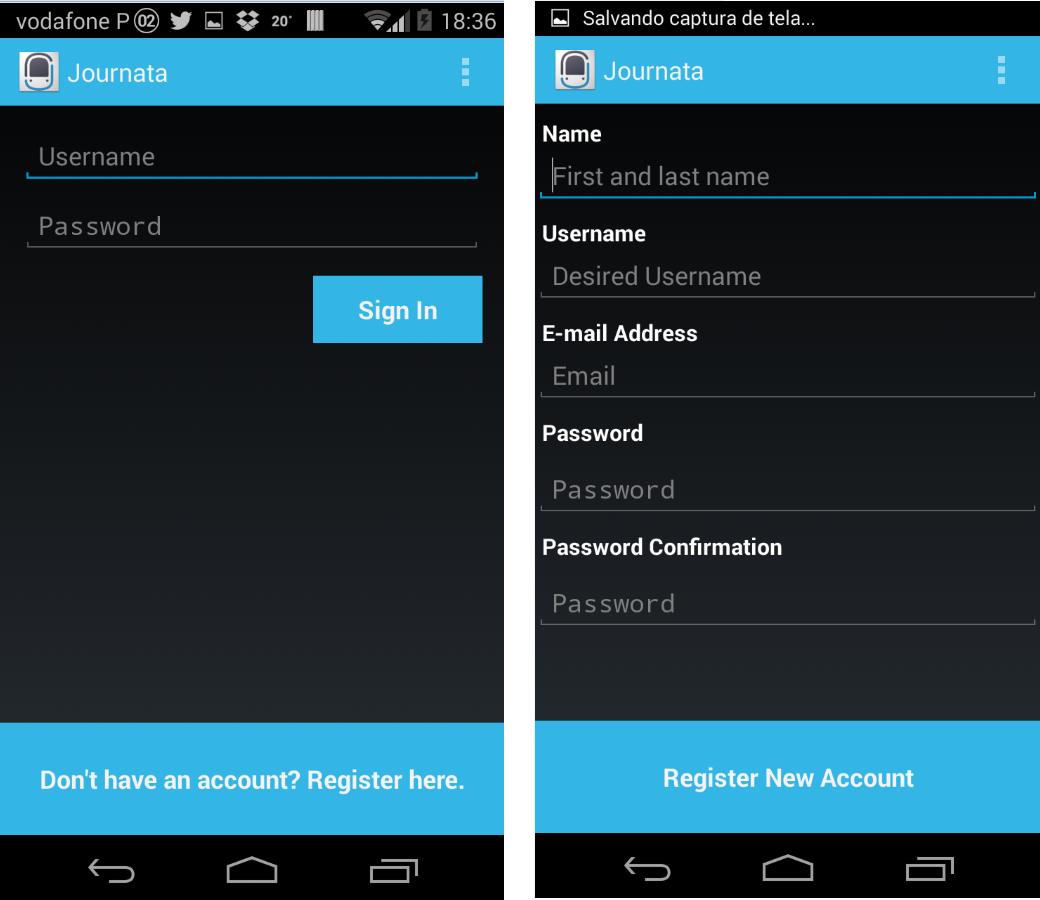
\includegraphics[scale=0.5]{login_register.png}
    \caption{Screenshots of the view feed feature (with refresh).}
    \label{fig:feed2}
  \end{center}
\end{figure}


Note that each comment has two buttons next to it, instead of the star that was part of the interfaces designed in previous iterations, and also that there are no highlighted comments prompting the user to rate them. This has been adapted due to changes in the point and rating system.

\subsubsection{Point System Redesign}

The limitations identified in section \ref{rateinitial}, alongside with the deprecation of \emph{Google Cloud to Device Messaging Framework}, that was beneath the previous existing rating system, led to the development of a whole new (and simpler) rating system, consisting in giving a 'thumbs up' or 'thumbs down' to a comment. Each 'thumbs up' adds one point to the score of the comment in question, while a 'thumbs down' subtracts one point from that score. That comment score is called 'feedback', and comments with negative feedback score are hidden from the news feed of other users. 

This also lead to a creation of a new field in the data structure referring to the user data: feedback points, which is the sum of the feedback score of all of the user's comments.

Those two buttons we can encounter to the right of the displayed comments in figure \ref{fig:feed2}, with the shape of an arrow, represent the 'thumbs up' and 'thumbs down' actions.

In order to display the right information, additional changes to the API were made. The existing implementation required an existing login and check-in in order to retrieve the set of information from a network, retrieving only the information for the network where the user was checked-in. Changes to that 'request' method had to be made in order to retrieve data from any network without those limitations.

\newpage

\subsection{Comment Submission}\label{comment}

\subsection{Authentication}\label{authentication}

Authentication is obviously present in the majority of applications, because most of them have features that require a creation of a user account.

All the effort of doing that, however, has been reduced in many applications, through allowing registration via an existing account for a known and widely used social network or type of account. For instance, it is fairly common to encounter an application where registering an account can be made using our \emph{Facebook}, \emph{Twitter} or \emph{Google} account. In theory, the implementation of authentication via \emph{Google} account will require less effort, within the mentioned options, because \emph{Android} users have a \emph{Google} account associated to their mobile device and are usually already authenticated in that account when using it.

The main concern about reducing the registration effort to the user is related with the possible risk of abandon. Having extensive registration forms reduced the user motivation to continue that process and create an account (and consequently, to use the application). That concern is even bigger in mobile applications, where text input is harder and prone to user errors (small-sized keys, allied in most cases to writing while performing other tasks, such as walking).

That said, minimizing the text input is the way to go when developing mobile applications. However, that is not enough.

One of the most important guidelines for the development of mobile applications is to avoid making users pass through a registration screen as a starting point to use the application. 
When a user starts using an application for the first time, he has a low level of commitment. Unless the application offers immense value to him, as quickly as possible, users won't use it enough to make registration worth their while. 

Forcing users to register before they are sufficiently convinced of the value provided by the application will probably cause many of them to simply back out from it and never try it again, therefore losing the chance of causing a first impression \cite{kn: MobileUsab}.

This guideline is not exactly new, as it is recommended since 1999 in e-commerce sites (a user should be able to buy items without having to register). Its importance, though, is greater in mobile applications, because every extra step that the user must pass through causes considerable effort, and users are less committed to an app they just downloaded than to a website where they have spent time browsing before being prompted to create an account.

\begin{quote}
"Registration on the first screen is an example of 'take before you give': Apps want users to spend time and effort without any perceived benefit. Asking for permission to send notifications of use the current location before users find out what the app is about is another way in which apps abuse their emerging relationship with the users. Often users have no idea of the purpose of those actions (...).' \cite{kn: MobileUsab}
\end{quote}


In the scope of this application, it was decided that the elimination of registration as a first step was one of the tasks with greater level of importance. That prompted another decision - what would be the features accessible to non-registered or non-authenticated users in order to give them some value before creating an account. 

The chosen features, given that the decoupling of the check-in requirement in order to receive network information was performed (as referred in section \ref{newsfeed}), were the ones related with the news feed component. That included adding new feeds, filter the information about the received feeds and to see the news feed information. 
Those features represent, for users that don't want to contribute with comments to the platform, a way to still receive the information they desire, possibly motivating them to contribute in the future if they wish to do it.

For the remaining features, those that require being logged in, a screen informing them to do so, along with a visible button that redirects them to the login screen, appears if they are not logged in yet. 

\begin{figure}[h!]
  \begin{center}
    \leavevmode
    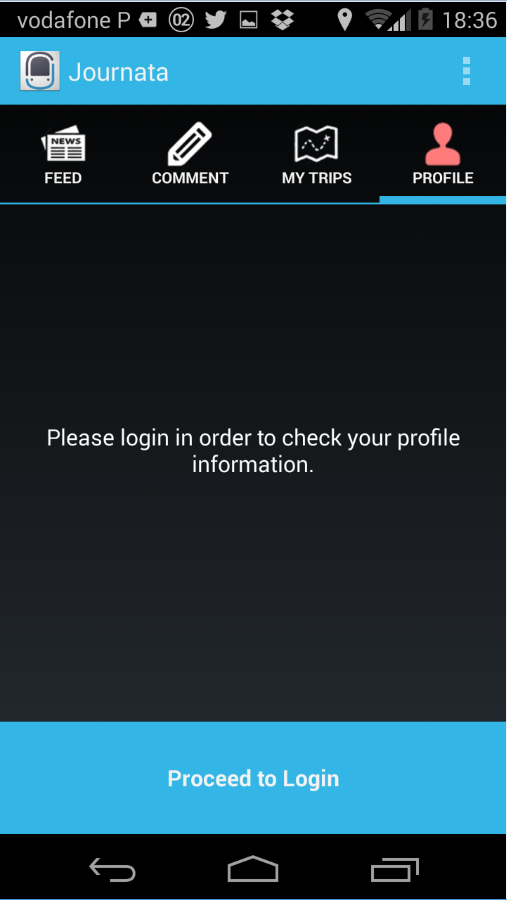
\includegraphics[scale=0.22]{profile_login.png}
    \caption{User profile screen - an example where authentication is required in order to access the information.}
    \label{fig:auth1}
  \end{center}
\end{figure}

In the login screen, a simple form asking for username and password is encountered, as well as the submit button for that form, and a button at the bottom of the screen that redirects the user for the register screen.

\begin{figure}[h!]
  \begin{center}
    \leavevmode
    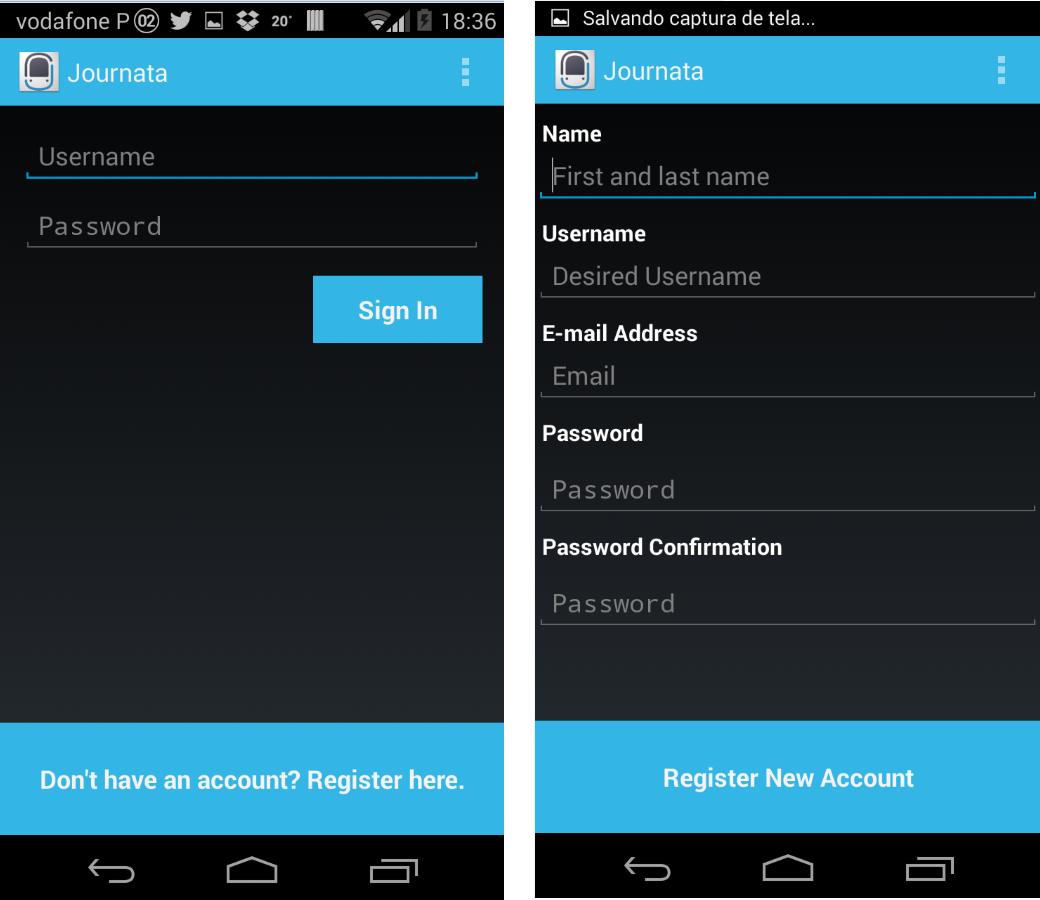
\includegraphics[scale=0.5]{login_register.png}
    \caption{Screenshots of the login and register screens.}
    \label{fig:auth2}
  \end{center}
\end{figure}

Other guidelines were followed in this process. The register form fields were reduced to the very essential - name, username, email, password and password confirmation - in order to reduce the text input effort from the user. The registration form in the previous prototype had two additional fields, nickname and the privacy setting. As for the first one, it may lead to a redundancy with the existing username field (when the privacy setting for the user is set as visible, instead of the nickname, the username field can be shown as there is no need for two distinct fields). 

Regarding the privacy setting, there is no need to define it so soon and introducing that effort on the registration form. Instead, it was assigned a default value for new accounts (public setting, but it can be easily modified in order to make that default the private setting) for the sake of demonstration in this prototype.

The submission of the registration form also triggers a login process after a successful registration. In short, after registering a new account, the user does not need to login and enter their data again, contrasting to what happened in the application developed in the previous iteration of the project.

The use of the \emph{Android} Action Bar as part of the interface allowed to create another options for logging in and logging out of the application, through the creation of an action menu where we can find login and logout buttons.

\begin{figure}[h!]
  \begin{center}
    \leavevmode
    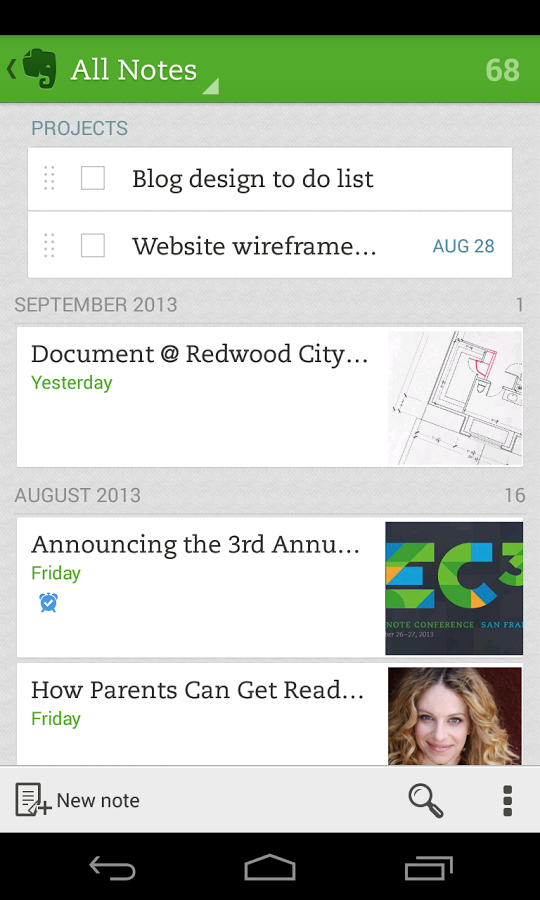
\includegraphics[scale=0.45]{auth1.png}
    \caption{Login and logout buttons in the Action Bar.}
    \label{fig:auth3}
  \end{center}
\end{figure}

Another concern during the development was the persistence of data after pausing or exiting the application. In the implementation of the prototype, all the data regarding the user login and profile is stored locally, in order to be accessible when entering the application again, after pausing or closing it. That said, the application does not require the user to login again after the first utilization (unless, of course, the user logs out in order to use other account).


\subsection{Journey Planner Features}\label{journeyplanner}

\subsection{User Profile}
